\documentclass[11p]{article}
% Packages
\usepackage{amsmath}
\usepackage{graphicx}
\usepackage[swedish]{babel}
\usepackage[
    backend=biber,
    style=authoryear-ibid,
    sorting=ynt
]{biblatex}
\usepackage[utf8]{inputenc}
\usepackage[T1]{fontenc}
%Källor
\addbibresource{mall.bib}


\title{PMmall   \small Fysik 1}
\author{Magnus Silverdal }
\date{\today}


\begin{document}

    \begin{titlepage}
        \begin{center}
            \vspace*{1cm}

            \Huge
            \textbf{Biomassa}

            \vspace{0.5cm}
            \LARGE
            Om miljö och samhällseffekterna av biomassa.

            \vspace{1.5cm}

            \textbf{Mille Tedebring Thysell}

            \vfill

            Ett PM om energiförsörjning  
            Fysik 1

            \vspace{0.8cm}

          %  \includegraphics[width=0.4\textwidth]{../images/NTI Gymnasiet_Symbol_print_svart.png}

            \Large
            Teknikprogrammet 
            NTI Gymnasiet 
            Umeå 
            \today

        \end{center}
    \end{titlepage}
% Om arbetet är långt har det en innehållsförteckning, annars kan den utelämnas
    \tableofcontents
    \newpage
    \section{Inledning}
    Biomassa är ett sätt att få energi från biologiska källor, specifikt växter, träd och generell plantmaterial.
    Biomassan har oftast formaten pellets eller flis som man får av överblivet material som inte kan användas till
    annat, detta kan man t.ex bränna för att få energi, man kan även använda bakterier för att få ut energin eller
    göra biomassan till en vätska. Biomassa är bra för att återfå energi av överblivet organiskt material som annars
    bara hade slängts, typ som sågspån, ogräs och generellt rensade plantmaterial.  \parencite{wikibiomassa}


    \section{Frågeställning}


     Fråga 1:
      
    
    Hur får man energi ur biomassa?


      Det finns tre sätt att få energi ur biomassa:
      Förbränning: Det simplaste sättet att få energi från biomassa är att bränna det och låta värmen
     koka vatten som sedan snurrar en turbin. Alltså typ exakt som kol och likt många andra kraftverk.
      Bakterier: Genom att använda organisk avfallsprodukt i en luftfri container så kan man låta specifika
     bakterier göra om det till metangas som kan användas som bränsle.
      Göra om det till gas/vätska: Genom att använda vissa processer så kan man göra om biomassan till en
     vätska eller gas och använda det som ett bränsle.

     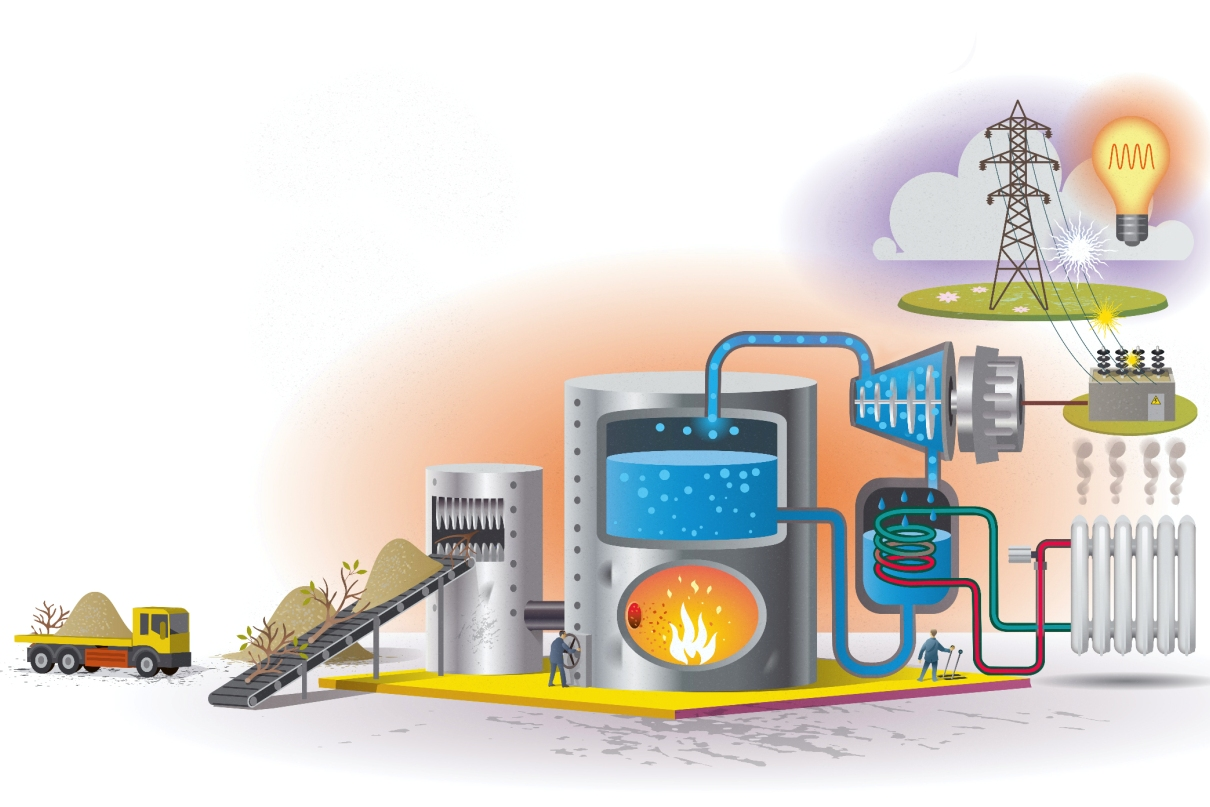
\includegraphics[scale=0.5]{kraftvarmeverk-1210x807}

       Fråga 2:
      Vilka miljöpåverkan har biomassa lokalt och globalt?
      Biomassa har likheter med fossila bränslen i hur man får energi ur det, men den stora skillnaden är
     att biomassa är förnybart. Plantmaterial växer konstant i stora mängder vilket gör att vi kan fortsätta
     använda det för evigt (teoretiskt).


      Fråga 3:
      Är biomassa hållbart för framtiden?
      Realistiskt så är biomassa inte en energikälla som vi enbart kan bero på, inte ens att en majoritet av
    vår energi kommer ifrån det. Detta är eftersom det tar väldigt lång tid för träd(största källan av biomassa)
    att växa, trä är den typen av biomassa som ger mest energi. \parencite{BiomassaVF}

\printbibliography
\end{document}
